\let\negmedspace\undefined
\let\negthickspace\undefined
\documentclass[journal]{IEEEtran}
\usepackage[a5paper, margin=10mm, onecolumn]{geometry}
\usepackage{tfrupee} 

\setlength{\headheight}{1cm} 
\setlength{\headsep}{0mm}  
\usepackage{gvv-book}
\usepackage{gvv}
\usepackage{cite}
\usepackage{amsmath,amssymb,amsfonts,amsthm}
\usepackage{algorithmic}
\usepackage{graphicx}
\usepackage{textcomp}
\usepackage{xcolor}
\usepackage{txfonts}
\usepackage{listings}
\usepackage{enumitem}
\usepackage{mathtools}
\usepackage{gensymb}
\usepackage{comment}
\usepackage[breaklinks=true]{hyperref}
\usepackage{tkz-euclide} 
\usepackage{listings}
% \usepackage{gvv}                                        
\def\inputGnumericTable{}                                 
\usepackage[latin1]{inputenc}                                
\usepackage{color}                                            
\usepackage{array}                                            
\usepackage{longtable}                                       
\usepackage{calc}                                             
\usepackage{multirow}                                         
\usepackage{hhline}                                           
\usepackage{ifthen}                                           
\usepackage{lscape}
\usepackage{tikz}
\usetikzlibrary{patterns}
\begin{document}

\bibliographystyle{IEEEtran}
\vspace{3cm}


\title{GATE 2021 ME }
\author{ee25btech11029- Jnanesh Sathisha Karmar}
\maketitle
% \maketitle
% \newpage
% \bigskip
{\let\newpage\relax\maketitle}

\renewcommand{\thefigure}{\theenumi}
\renewcommand{\thetable}{\theenumi}
\setlength{\intextsep}{10pt} % Space between text and floats
\textbf{Q0.1 - Q0.5 Multiple Choice Question (MCQ), carry ONE mark each (for each wrong answer: - 1/3 ) .}
\begin{enumerate}[leftmargin=0pt]

\item Consider the following sentences:
\begin{enumerate}
\item After his surgery, Raja hardly could walk.
\item After his surgery, Raja could barely walk.
\item After his surgery, Raja barely could walk.
\item After his surgery, Raja could hardly walk.
\end{enumerate}

Which of the above sentences are grammatically CORRECT?

\begin{enumerate}
\begin{multicols}{4}
\item \brak{\text{(i) and (ii)}}
\item \brak{\text{(i) and (iii)}}
\item \brak{\text{(iii) and (iv)}}
\item \brak{\text{(ii) and (iv)}}
\end{multicols}
\end{enumerate}

\hfill{\brak{\text{GATE ME 2021}}}

\item Ms. X came out of a building through its front door to find her shadow due
to the morning sun falling to her right side with the building to her back.
From this, it can be inferred that building is facing \underline{\hspace{2cm}}.

\begin{enumerate}
\begin{multicols}{4}
\item \brak{\text{North}}
\item \brak{\text{East}}
\item \brak{\text{West}}
\item \brak{\text{South}}
\end{multicols}
\end{enumerate}

\hfill{\brak{\text{GATE ME 2021}}}

\item 
\begin{figure}[h]
\centering
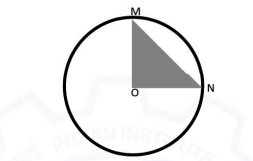
\includegraphics[width=0.5\columnwidth]{Figs/image (34).png}
\caption*{}
\label{fig:3}
\end{figure}
In the above figure, O is the center of the circle and, M and N lie on the
circle.

The area of the right triangle MON is $50 \text{ cm}^2$.

What is the area of the circle in $\text{cm}^2$?

\begin{enumerate}
\begin{multicols}{4}
\item $2 \pi$
\item $50 \pi$
\item $75 \pi$
\item $100 \pi$
\end{multicols}
\end{enumerate}

\hfill{\brak{\text{GATE ME 2021}}}

\item ''-'' means $-$, ''+'' means $+$, If
''$\triangle$'' means $+$ , ''$\nabla$'' means $\times$ ,

then, the value of the expression $\triangle 2 \oplus 3 \triangle ((42) \nabla 4)$ =

\begin{enumerate}
\begin{multicols}{4}
\item $-1$
\item $-0.5$
\item $6$
\item $7$
\end{multicols}
\end{enumerate}

\hfill{\brak{\text{GATE ME 2021}}}

\item ``The increased consumption of leafy vegetables in the recent months is a
clear indication that the people in the state have begun to lead a healthy
lifestyle"

Which of the following can be logically inferred from the information
presented in the above statement?

\begin{enumerate}

\item \brak{\text{The people in the state did not consume leafy vegetables earlier.}}
\item \brak{\text{Consumption of leafy vegetables may not be the only indicator of healthy
lifestyle.}}
\item \brak{\text{Leading a healthy lifestyle is related to a diet with leafy vegetables.}}
\item \brak{\text{The people in the state have increased awareness of health hazards causing by
consumption of junk foods.}}

\end{enumerate}

\hfill{\brak{\text{GATE ME 2021}}}
\textbf{Q. 6-Q. 10 Multiple Choice Question (MCQ), carry TWO marks each (for each wrong answer: 2/3).}

\item Oxpeckers and rhinos manifest a symbiotic relationship in the wild. The
oxpeckers warn the rhinos about approaching poachers, thus possibly
saving the lives of the rhinos. Oxpeckers also feed on the parasitic ticks
found on rhinos.

In the symbiotic relationship described above, the primary benefits for
oxpeckers and rhinos respectively are,

\begin{enumerate}

\item \brak{\text{Oxpeckers get a food source, rhinos have no benefit.}}
\item \brak{\text{Oxpeckers save their habitat from poachers while the rhinos have no benefit.}}
\item \brak{\text{Oxpeckers get a food source, rhinos may be saved from the poachers.}}
\item \brak{\text{Oxpeckers save the lives of poachers, rhinos save their own lives.}}

\end{enumerate}

\hfill{\brak{\text{GATE ME 2021}}}

\item
\begin{figure}[h]
\centering
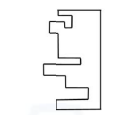
\includegraphics[width=0.5\columnwidth]{Figs/image (35).png}
\caption*{}
\label{fig:7}
\end{figure}
A jigsaw puzzle has 2 pieces. One of the pieces is shown above. Which one of
the given options for the missing piece when assembled will form a
rectangle? The piece can be moved, rotated or flipped to assemble with the
above piece.

\begin{enumerate}

\item 
\begin{figure}[h]
\centering
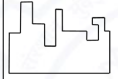
\includegraphics[width=0.1\columnwidth]{Figs/image (36).png}
\caption*{}
\label{fig:a}
\end{figure}
\item 
\begin{figure}[h]
\centering
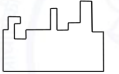
\includegraphics[width=0.1\columnwidth]{Figs/image (37).png}
\caption*{}
\label{fig:b}
\end{figure}
\item 
\begin{figure}[h]
\centering
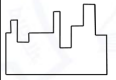
\includegraphics[width=0.1\columnwidth]{Figs/image (38).png}
\caption*{}
\label{fig:c}
\end{figure}
\item
\begin{figure}[h]
\centering
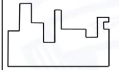
\includegraphics[width=0.1\columnwidth]{Figs/image (39).png}
\caption*{}
\label{fig:d}
\end{figure}

\end{enumerate}

\hfill{\brak{\text{GATE ME 2021}}}

\item The number of hens, ducks and goats in farm P are $65, 91$ and $169$,
respectively. The total number of hens, ducks and goats in a nearby farm Q
is $416$. The ratio of hens:ducks:goats in farm Q is $5:14:13$. All the hens, ducks and goats are sent from farm Q to farm P.

The new ratio of hens:ducks:goats in farm P is

\begin{enumerate}
\begin{multicols}{4}
\item $5:7:13$
\item $5:14:13$
\item $10:21:26$
\item $21:10:26$
\end{multicols}
\end{enumerate}

\hfill{\brak{\text{GATE ME 2021}}}

\item 
\begin{figure}[h]
\centering
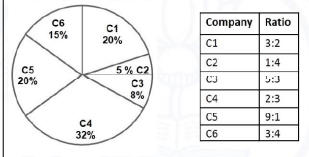
\includegraphics[width=0.5\columnwidth]{Figs/image (40).png}
\caption*{}
\label{fig:9}
\end{figure}
\newpage
The distribution of employees at the rank of executives, across different
companies C1, C2, ..., C6 is presented in the chart given above. The ratio of
executives with a management degree to those without a management degree
in each of these companies is provided in the table above. The total number
of executives across all companies is $10,000$.

The total number of management degree holders among the executives in
companies C2 and C5 together is \underline{\hspace{2cm}}.

\hfill{\brak{\text{GATE ME 2021}}}

\item Five persons P, Q, R, S and T are sitting in a row not necessarily in the same
order. Q and R are separated by one person, and S should not be seated
adjacent to Q.

The number of distinct seating arrangements possible is:

\begin{enumerate}
\begin{multicols}{4}
\item $4$
\item $8$
\item $10$
\item $16$
\end{multicols}
\end{enumerate}

\hfill{\brak{\text{GATE ME 2021}}}
\end{enumerate}
\textbf{Q.1-Q.19 Multiple Choice Question (MCQ), carry ONE mark each (for each wrong answer: 1/3).}
\begin{enumerate}
\item If $y(x)$ satisfies the differential equation
\[
\frac{d}{dx}(\sin x) + y \cos x = 1,
\]
subject to the condition $y(\pi/2) = \pi/2$, then $y(\pi/6)$ is

\begin{enumerate}
\begin{multicols}{4}
\item $0$
\item $\frac{\pi}{6}$
\item $\frac{\pi}{3}$
\item $\frac{\pi}{2}$
\end{multicols}
\end{enumerate}

\hfill{\brak{\text{GATE ME 2021}}}

\item The value of $\lim_{x \to 0} \frac{1-\cos x}{x^2}$ is

\begin{enumerate}
\begin{multicols}{4}
\item $\frac{1}{4}$
\item $\frac{1}{3}$
\item $\frac{1}{2}$
\item $1$
\end{multicols}
\end{enumerate}

\hfill{\brak{\text{GATE ME 2021}}}

\item The Dirac-delta function $\delta(t - t_0)$ for $t, t_0 \in \mathbb{R}$, has the following property
\[
\int_a^b \phi(t) \delta(t - t_0) dt =
\begin{cases}
\phi(t_0), & a < t_0 < b \\
0, & \text{otherwise}
\end{cases}
\]

The Laplace transform of the Dirac-delta function $\delta(t - a)$ for $a > 0$;
$L(\delta(t - a)) = F(s)$ is

\begin{enumerate}
\begin{multicols}{4}
\item $0$
\item $\infty$
\item $e^{sa}$
\item $e^{-sa}$
\end{multicols}
\end{enumerate}

\hfill{\brak{\text{GATE ME 2021}}}

\item The ordinary differential equation
\[
\frac{dy}{dt} = -\pi y,
\]
subject to an initial condition $y(0) = 1$ is solved numerically using the following scheme,
\[
\frac{y(t_{n+1}) - y(t_n)}{h} = -\pi y(t_n),
\]
where $h$ is the time step, $t_n = nh$, and $n = 0, 1, 2, \dots$. This numerical scheme
is stable for all values of $h$ in the interval

\begin{enumerate}
\begin{multicols}{4}
\item $0 < h < \frac{2}{\pi}$
\item $0 < h < 1$
\item $0 < h < \frac{\pi}{2}$
\item \text{for all } $h > 0$
\end{multicols}
\end{enumerate}

\hfill{\brak{\text{GATE ME 2021}}}

\item Consider a binomial random variable $X$. If $X_1, X_2, \ldots, X_n$ are independent and identically distributed samples from the distribution of $X$ with sum $Y = \sum_i X_i$, then the distribution of $Y$ as $n \rightarrow \infty$ can be approximated as

\begin{enumerate}
\begin{multicols}{4}
\item Exponential
\item Bernoulli
\item Binomial
\item Normal
\end{multicols}
\end{enumerate}

\hfill{\brak{\text{GATE ME 2021}}}

\item
\begin{figure}[h]
\centering
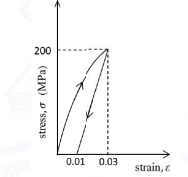
\includegraphics[width=0.5\columnwidth]{Figs/image (41).png}
\caption*{}
\label{fig:6}
\end{figure}
The loading and unloading response of a metal is shown in the figure. The elastic and plastic strains corresponding to $200 \text{ MPa}$ stress, respectively, are

\begin{enumerate}
\begin{multicols}{4}
\item $0.01$ and $0.01$
\item $0.02$ and $0.01$
\item $0.01$ and $0.02$
\item $0.02$ and $0.02$
\end{multicols}
\end{enumerate}

\hfill{\brak{\text{GATE ME 2021}}}

\item 

In a machining operation, if a cutting tool traces the workpiece such that the
directrix is perpendicular to the plane of the generatrix as shown in figure,
the surface generated is
\begin{figure}[h]
\centering
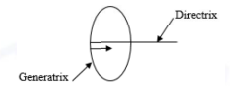
\includegraphics[width=0.5\columnwidth]{Figs/image (42).png}
\caption*{}
\label{fig:7}
\end{figure}

\begin{enumerate}
\begin{multicols}{2}
\item plane
\item cylindrical
\item spherical
\item a surface of revolution
\end{multicols}
\end{enumerate}

\hfill{\brak{\text{GATE ME 2021}}}

\item The correct sequence of machining operations to be performed to finish a
large diameter through hole is

\begin{enumerate}
\begin{multicols}{4}
\item drilling, boring, reaming
\item boring, drilling, reaming
\item drilling, reaming, boring
\item boring, reaming, drilling
\end{multicols}
\end{enumerate}

\hfill{\brak{\text{GATE ME 2021}}}

\item In modern CNC machine tools, the backlash has been eliminated by

\begin{enumerate}
\begin{multicols}{2}
\item preloaded ballscrews
\item rack and pinion
\item ratchet and pinion
\item slider crank mechanism
\end{multicols}
\end{enumerate}

\hfill{\brak{\text{GATE ME 2021}}}

\item Consider the surface roughness profile as shown in the figure.
\begin{figure}[h]
\centering
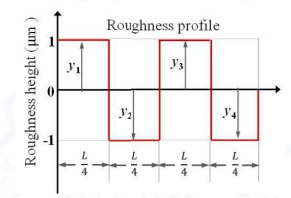
\includegraphics[width=0.5\columnwidth]{Figs/image (43).png}
\caption*{}
\label{fig:10}
\end{figure}
\newpage
The center line average roughness $(R_a$, in $\mu m)$ of the measured length $(L)$ is

\begin{enumerate}
\begin{multicols}{4}
\item $0$
\item $1$
\item $2$
\item $4$
\end{multicols}
\end{enumerate}

\hfill{\brak{\text{GATE ME 2021}}}

\item In which of the following pairs of cycles, both cycles have at least one isothermal process?

\begin{enumerate}
\begin{multicols}{2}
\item Diesel cycle and Otto cycle
\item Carnot cycle and Stirling cycle
\item Brayton cycle and Rankine cycle
\item Bell-Coleman cycle and Vapour compression refrigeration cycle
\end{multicols}
\end{enumerate}

\hfill{\brak{\text{GATE ME 2021}}}




\item Superheated steam at $1500$ kPa, has a specific volume of $2.75~\text{m}^3/\text{kmol}$ and compressibility factor $(Z)$ of $0.95$. The temperature of steam is \underline{\hspace{2cm}}~$^\degree$C (\text{round off to the nearest integer}).

\begin{enumerate}
\begin{multicols}{4}
\item $522$
\item $471$
\item $249$
\item $198$
\end{multicols}
\end{enumerate}

\hfill{\brak{\text{GATE ME 2021}}}

\item A hot steel spherical ball is suddenly dipped into a low temperature oil bath. Which of the following dimensionless parameters are required to determine instantaneous center temperature of the ball using a Heisler chart?

\begin{enumerate}
\begin{multicols}{2}
\item Biot number and Fourier number
\item Reynolds number and Prandtl number
\item Biot number and Froude number
\item Nusselt number and Grashoff number
\end{multicols}
\end{enumerate}

\hfill{\brak{\text{GATE ME 2021}}}

\item An infinitely long pin fin, attached to an isothermal hot surface, transfers heat at a steady rate of $Q_1$ to the ambient air. If the thermal conductivity of the fin material is doubled, while keeping everything else constant, the rate of steady-state heat transfer from the fin becomes $Q_2$. The ratio $\frac{Q_2}{Q_1}$ is

\begin{enumerate}
\begin{multicols}{2}
\item $\sqrt{2}$
\item $2$
\item $\frac{1}{\sqrt{2}}$
\item $\frac{1}{2}$
\end{multicols}
\end{enumerate}

\hfill{\brak{\text{GATE ME 2021}}}


\item The relative humidity of ambient air at $300~\text{K}$ is $50\%$ with a partial pressure of water vapour equal to $p_v$. The saturation pressure of water at $300~\text{K}$ is $p_{sat}$. The correct relation for the air-water mixture is

\begin{enumerate}
\begin{multicols}{2}
\item $p_v = 0.5\, p_{sat}$
\item $p_v = p_{sat}$
\item $p_v = 0.622\, p_{sat}$
\item $p_v = 2\, p_{sat}$
\end{multicols}
\end{enumerate}

\hfill{\brak{\text{GATE ME 2021}}}

\item Consider a reciprocating engine with crank radius $R$ and connecting rod of length $L$. The secondary unbalance force for this case is equivalent to primary unbalance force due to a virtual crank of $\underline{\hspace{2cm}}$.

\begin{enumerate}
\begin{multicols}{2}
\item radius $\frac{L^2}{4R}$ rotating at half the engine speed
\item radius $\frac{R}{4}$ rotating at half the engine speed
\item radius $\frac{R^2}{4L}$ rotating at twice the engine speed
\item radius $\frac{L}{2}$ rotating at twice the engine speed
\end{multicols}
\end{enumerate}

\hfill{\brak{\text{GATE ME 2021}}}



\item A cantilever beam of length, $L$, and flexural rigidity, $EI$, is subjected to an end moment, $M$, as shown in the figure. The deflection of the beam at $x = \frac{L}{2}$ is
\begin{figure}[h]
\centering
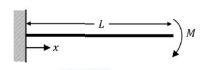
\includegraphics[width=0.5\columnwidth]{Figs/image (44).png}
\caption*{}
\label{fig:17}
\end{figure}

\begin{enumerate}
\begin{multicols}{2}
\item $\frac{ML^2}{2EI}$
\item $\frac{ML^2}{4EI}$
\item $\frac{ML^2}{8EI}$
\item $\frac{ML^2}{16EI}$
\end{multicols}
\end{enumerate}

\hfill{\brak{\text{GATE ME 2021}}}

\item A prismatic bar $PQRST$ is subjected to axial loads as shown in the figure. The segments having maximum and minimum axial stresses, respectively, are
\begin{figure}[h]
\centering
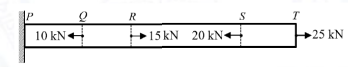
\includegraphics[width=0.5\columnwidth]{Figs/image (45).png}
\caption*{}
\label{fig:18}
\end{figure}
\newpage

\begin{enumerate}
\begin{multicols}{2}
\item $QR$ and $PQ$
\item $ST$ and $PQ$
\item $QR$ and $RS$
\item $ST$ and $RS$
\end{multicols}
\end{enumerate}

\hfill{\brak{\text{GATE ME 2021}}}


\item Shear stress distribution on the cross-section of the coil wire in a helical compression spring is shown in the figure. This shear stress distribution represents
\begin{figure}[h]
\centering
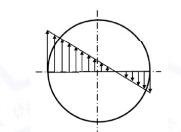
\includegraphics[width=0.5\columnwidth]{Figs/image (46).png}
\caption*{}
\label{fig:19}
\end{figure}

\begin{enumerate}
\begin{multicols}{2}
\item direct shear stress in the coil wire cross-section
\item torsional shear stress in the coil wire cross-section
\item combined direct shear and torsional shear stress in the coil wire cross-section
\item combined direct shear and torsional shear stress along with the effect of stress concentration at inside edge of the coil wire cross-section
\end{multicols}
\end{enumerate}

\hfill{\brak{\text{GATE ME 2021}}}

\textbf{Q.20-Q.25 Numerical Answer Type (NAT), carry ONE mark each (no negative marks).}

\item Robot Ltd. wishes to maintain enough safety stock during the lead time period between starting a new production run and its completion such that the probability of satisfying the customer demand during the lead time period is $95\%$. The lead time period is $5$ days and daily customer demand can be assumed to follow the Gaussian (normal) distribution with mean $50$ units and a standard deviation of $10$ units. Using $\Phi^{-1}(0.95) = 1.64$, where $\Phi$ represents the cumulative distribution function of the standard normal random variable, the amount of safety stock that must be maintained by Robot Ltd. to achieve this demand fulfillment probability for the lead time period is \underline{\hspace{2cm}} units (\text{round off to two decimal places}).

\hfill{\brak{\text{GATE ME 2021}}}

\item A pressure measurement device fitted on the surface of a submarine, located at a depth $H$ below the surface of an ocean, reads an absolute pressure of $4.2$ MPa. The density of sea water is $1050$ kg/m$^3$, the atmospheric pressure is $101$ kPa, and the acceleration due to gravity is $9.8$ m/s$^2$. The depth $H$ is \underline{\hspace{2cm}} m (\text{round off to the nearest integer}).

\hfill{\brak{\text{GATE ME 2021}}}

\item Consider fully developed, steady state incompressible laminar flow of a viscous fluid between two large parallel horizontal plates. The bottom plate is fixed and the top plate moves with a constant velocity of $U = 4$ m/s. Separation between the plates is $5$ mm. There is no pressure gradient in the direction of flow. The density of fluid is $800$ kg/m$^3$, and the kinematic viscosity is $1.25 \times 10^{-4}$ m$^2$/s. The average shear stress in the fluid is \underline{\hspace{2cm}} Pa (\text{round off to the nearest integer}).

\hfill{\brak{\text{GATE ME 2021}}}

\item A rigid insulated tank is initially evacuated. It is connected through a valve to a supply line that carries air at a constant pressure and temperature of $250$ kPa and $400$ K respectively. Now the valve is opened and air is allowed to flow into the tank until the pressure inside the tank reaches $250$ kPa at which point the valve is closed. Assume that the air behaves as a perfect gas with constant properties $(C_p = 1.005\, \text{kJ/kg.K}, c_v = 0.718\, \text{kJ/kg.K}, R = 0.287\, \text{kJ/kg.K})$. Final temperature of the air inside the tank is \underline{\hspace{2cm}} K (\text{round off to one decimal place}).

\hfill{\brak{\text{GATE ME 2021}}}

\item The figure shows an arrangement of a heavy propeller shaft in a ship. The combined polar mass moment of inertia of the propeller and the shaft is $100$ kg$\cdot$m$^2$. The propeller rotates at $\omega = 12$ rad/s. The waves acting on the ship hull induces a rolling motion as shown in the figure with an angular velocity of $5$ rad/s. The gyroscopic moment generated on the shaft due to the motion described is \underline{\hspace{2cm}} N$\cdot$m (\text{round off to the nearest integer}).
\begin{figure}[h]
\centering
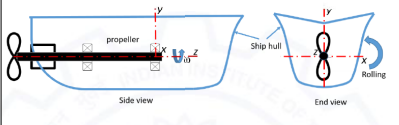
\includegraphics[width=0.5\columnwidth]{Figs/image (47).png}
\caption*{}
\label{fig:24}
\end{figure}

\hfill{\brak{\text{GATE ME 2021}}}

\item Consider a single degree of freedom system comprising a mass $M$, supported on a spring and a dashpot as shown in the figure.
\begin{figure}[h]
\centering
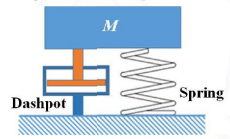
\includegraphics[width=0.5\columnwidth]{Figs/image (48).png}
\caption*{}
\label{fig:25}
\end{figure}

If the amplitude of the free vibration response reduces from $8$ mm to $1.5$ mm in $3$ cycles, the damping ratio of the system is \underline{\hspace{2cm}} (\text{round off to three decimal places}).

\hfill{\brak{\text{GATE ME 2021}}}
\textbf{Q. 26-Q. 34 Multiple Choice Question (MCQ), carry TWO mark each (for each wrong answer: 2/3).}
\item Consider a vector $p$ in $2$-dimensional space. Let its direction (counterclockwise angle with the positive $x$-axis) be $\theta$. Let $p$ be an eigenvector of a $2 \times 2$ matrix $A$ with corresponding eigenvalue $\lambda$, $\lambda>0$. If we denote the magnitude of a vector $v$ by $\abs{v}$, identify the VALID statement regarding $p'$, where $p' = Ap$.

\begin{enumerate}
\begin{multicols}{2}
\item Direction of $p' = \lambda\theta$, $\abs{p'} = \abs{p}$
\item Direction of $p' = \theta$, $\abs{p'} = \lambda\abs{p}$
\item Direction of $p' = \lambda\theta$, $\abs{p'} = \lambda\abs{p}$
\item Direction of $p' = \theta$, $\abs{p'} = \abs{p}/\lambda$
\end{multicols}
\end{enumerate}

\hfill{\brak{\text{GATE ME 2021}}}

\item Let $C$ represent the unit circle centered at origin in the complex plane, and complex variable, $z = x + iy$. The value of the contour integral
\[
\oint_C \frac{\cosh 3z}{2z} dz
\]
(where integration is taken counter clockwise) is

\begin{enumerate}
\begin{multicols}{2}
\item $0$
\item $2$
\item $\pi i$
\item $2\pi i$
\end{multicols}
\end{enumerate}

\hfill{\brak{\text{GATE ME 2021}}}


\item A set of jobs $A, B, C, D, E, F, G, H$ arrive at time $t=0$ for processing on turning and grinding machines. Each job needs to be processed in sequence - first on the turning machine and second on the grinding machine, and the grinding must occur immediately after turning. The processing times of the jobs are given below.


\begin{table}[h!]
\caption*{}
\label{tab:job_processing}
\begin{tabular}{c|cccccccc}
Job & A & B & C & D & E & F & G & H \\
\hline
Turning (minutes) & 2 & 4 & 8 & 9 & 7 & 6 & 5 & 10 \\
Grinding (minutes) & 6 & 1 & 3 & 7 & 9 & 5 & 2 & 4 \\
\end{tabular}
\end{table}

If the makespan is to be minimized, then the optimal sequence in which these jobs must be processed on the turning and grinding machines is

\begin{enumerate}
\begin{multicols}{2}
\item A-E-D-F-H-C-G-B
\item A-D-E-F-H-C-G-B
\item G-E-D-F-H-C-A-B
\item B-G-C-H-F-D-E-A
\end{multicols}
\end{enumerate}

\hfill{\brak{\text{GATE ME 2021}}}

\item The fundamental thermodynamic relation for a rubber band is given by $dU = TdS + \tau dL$, where $T$ is the absolute temperature, $S$ is the entropy, $\tau$ is the tension in the rubber band, and $L$ is the length of the rubber band. Which one of the following relations is CORRECT:

\begin{enumerate}
\begin{multicols}{2}
\item $\tau = \left(\frac{\partial U}{\partial L}\right)_S$
\item $\tau = \left(\frac{\partial T}{\partial S}\right)_L$
\item $T = \left(\frac{\partial \tau}{\partial S}\right)_L$
\item $T = \left(\frac{\partial U}{\partial S}\right)_\tau$
\end{multicols}
\end{enumerate}

\hfill{\brak{\text{GATE ME 2021}}}

\item Consider a two degree of freedom system as shown in the figure, where $PQ$ is a rigid uniform rod of length $b$ and mass $m$. Assume that the spring deflects only horizontally and force $F$ is applied horizontally at $Q$. For this system, the Lagrangian, $L$ is
\begin{figure}[h]
\centering
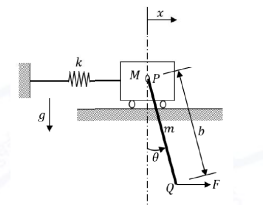
\includegraphics[width=0.5\columnwidth]{Figs/image (50).png}
\caption*{}
\label{fig:30}
\end{figure}
\begin{enumerate}
\begin{multicols}{2}
\item $\frac{1}{2}(M+m)\dot{x}^2 + \frac{1}{6}mb^2\dot{\theta}^2 - \frac{1}{2}kx^2 + mg\cos\theta$
\item $\frac{1}{2}(M+m)\dot{x}^2 + \frac{1}{2}mb^2\dot{\theta}^2 - kx^2 + mg\cos\theta + b\cos\theta$
\item $\frac{1}{2}M\dot{x}^2 + \frac{1}{2}mb\dot{x}\cos\theta + \frac{1}{6}mb^2\dot{\theta}^2 - \frac{1}{2}kx^2$
\item $\frac{1}{2}M\dot{x}^2 + \frac{1}{2}mb\dot{x}\cos\theta + \frac{1}{6}mb^2\dot{\theta}^2 - \frac{1}{2}kx^2 + b\cos\theta + Fb\sin\theta$
\end{multicols}
\end{enumerate}

\hfill{\brak{\text{GATE ME 2021}}}

\item A right solid circular cone standing on its base on a horizontal surface is of height $H$ and base radius $R$. The cone is made of a material with specific weight $w$ and elastic modulus $E$. The vertical deflection at the mid-height of the cone due to self-weight is given by

\begin{enumerate}
\begin{multicols}{2}
\item $\frac{wH^2}{8E}$
\item $\frac{wH^2}{6E}$
\item $\frac{wRH}{8E}$
\item $\frac{wRH}{6E}$
\end{multicols}
\end{enumerate}

\hfill{\brak{\text{GATE ME 2021}}}

\item A tappet valve mechanism in an IC engine comprises a rocker arm $ABC$ that is hinged at $B$ as shown in the figure. The rocker is assumed rigid and it oscillates about the hinge $B$. The mass moment of inertia of the rocker about $B$ is $10^4~\text{kg m}^2$. The rocker arm dimensions are $a = 3.5$~cm and $b = 2.5$~cm. A pushrod pushes the rocker at location $A$, when moved vertically by a cam that rotates at $N$ rpm. The pushrod is assumed massless and has a stiffness of $15$~N/mm. At the other end $C$, the rocker pushes a valve against a spring of stiffness $10$~N/mm. The valve is assumed massless and rigid.
\begin{figure}[h]
\centering
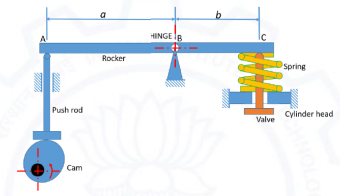
\includegraphics[width=0.5\columnwidth]{Figs/image (51).png}
\caption*{}
\label{fig:32}
\end{figure}
Resonance in the rocker system occurs when the cam shaft runs at a speed \underline{\hspace{2cm}} rpm (\text{round off to the nearest integer}).

\begin{enumerate}
\begin{multicols}{2}
\item $496$
\item $4739$
\item $790$
\item $2369$
\end{multicols}
\end{enumerate}

\hfill{\brak{\text{GATE ME 2021}}}



\item Customers arrive at a shop according to the Poisson distribution with a mean of $10$ customers/hour. The manager notes that no customer arrives for the first $3$ minutes after the shop opens. The probability that a customer arrives within the next $3$ minutes is

\begin{enumerate}
\begin{multicols}{2}
\item $0.39$
\item $0.86$
\item $0.50$
\item $0.61$
\end{multicols}
\end{enumerate}

\hfill{\brak{\text{GATE ME 2021}}}

\item Let $f(x) = x^2 - 2x + 2$ be a continuous function defined on $x \in [1,3]$.
The point $x$ at which the tangent of $f(x)$ becomes parallel to the straight line joining $f(1)$ and $f(3)$ is

\begin{enumerate}
\begin{multicols}{2}
\item $0$
\item $1$
\item $2$
\item $3$
\end{multicols}
\end{enumerate}

\hfill{\brak{\text{GATE ME 2021}}}
\textbf{Mechanical Engineering (ME, Set-1)
Q.35-Q.55 Numerical Answer Type (NAT), carry TWO mark each (no negative marks).}
\item Activities A, B, C and D form the critical path for a project with a PERT
network. The means and variances of the activity duration for each activity
are given below. All activity durations follow the Gaussian (normal)
distribution, and are independent of each other.

\begin{table}[h!]
\caption*{}
\label{tab:pert_project}
\begin{tabular}{|c|c|c|c|c|}
\hline
Activity & A & B & C & D \\
\hline
Mean (days) & 6 & 11 & 8 & 15 \\
\hline
Variance (days$^2$) & 4 & 9 & 4 & 9 \\
\hline
\end{tabular}
\end{table}

The probability that the project will be completed within $40$ days is \underline{\hspace{2cm}} (round off to two decimal places).

\hfill{\brak{\text{GATE ME 2021}}}

\item A true centrifugal casting operation needs to be performed horizontally to
make copper tube sections with outer diameter of $250$ mm and inner
diameter of $230$ mm. The value of acceleration due to gravity, $g=10$ m/s$^2$.
If a G-factor (ratio of centrifugal force to weight) of $60$ is used for casting
the tube, the rotational speed required is \underline{\hspace{2cm}} rpm (round off to the nearest integer).

\hfill{\brak{\text{GATE ME 2021}}}

\item The resistance spot welding of two $1.55$ mm thick metal sheets is performed
using welding current of $10000$ A for $0.25$ s. The contact resistance at the
interface of the metal sheets is $0.0001~\ohm$. The volume of weld nugget formed after welding is $70$ mm$^3$. Considering the heat required to melt unit volume of metal is $12$ J/mm$^3$, the thermal efficiency of the welding process is \underline{\hspace{2cm}} \% (round off to one decimal place).

\hfill{\brak{\text{GATE ME 2021}}}

\item An orthogonal cutting operation is performed using a single point cutting
tool with a rake angle of $12^\degree$ on a lathe. During turning, the cutting force and the friction force are $1000$ N and $600$ N, respectively. If the chip thickness and the uncut chip thickness during turning are $1.5$ mm and $0.75$ mm, respectively, then the shear force is \underline{\hspace{2cm}} N (round off to two decimal places).

\hfill{\brak{\text{GATE ME 2021}}}

\item In a grinding operation of a metal, specific energy consumption is $15$ J/mm$^3$. If a grinding wheel with a diameter of $200$ mm is rotating at $3000$ rpm to obtain a material removal rate of $6000$ mm$^3$/min, then the tangential force on the wheel is \underline{\hspace{2cm}} N (round off to two decimal places).

\hfill{\brak{\text{GATE ME 2021}}}

\item A $200$ mm wide plate having a thickness of $20$ mm is fed through a rolling
mill with two rolls. The radius of each roll is $300$ mm. The plate thickness is to be reduced to $18$ mm in one pass using a roll speed of $50$ rpm. The strength coefficient $(K)$ of the work material flow curve is $300$ MPa and the strain hardening exponent, $n$ is $0.2$. The coefficient of friction between the rolls and the plate is $0.1$. If the friction is sufficient to permit the rolling operation then the roll force will be \underline{\hspace{2cm}} kN (round off to the nearest integer).

\hfill{\brak{\text{GATE ME 2021}}}

\item The XY table of a NC machine tool is to move from $P(1,1)$ to $Q(51,1)$; all coordinates are in mm. The pitch of the NC drive leadscrew is $1$ mm. If the backlash between the leadscrew and the nut is $1.8^\degree$, then the total backlash of the table on moving from $P$ to $Q$ is \underline{\hspace{2cm}} mm (round off to two decimal places).

\hfill{\brak{\text{GATE ME 2021}}}

\item Consider a single machine workstation to which jobs arrive according to a Poisson distribution with a mean arrival rate of $12$ jobs/hour. The process time of the workstation is exponentially distributed with a mean of $4$ minutes. The expected number of jobs at the workstation at any given point of time is \underline{\hspace{2cm}} (round off to the nearest integer).

\hfill{\brak{\text{GATE ME 2021}}}

\item An uninsulated cylindrical wire of radius $1.0$ mm produces electric heating at the rate of $5.0$ W/m. The temperature of the surface of the wire is $75^\degree$C when placed in air at $25^\degree$C. When the wire is coated with PVC of thickness $1.0$ mm, the temperature of the surface of the wire reduces to $55^\degree$C. Assume that the heat generation rate from the wire and the convective heat transfer coefficient are same for both uninsulated wire and the coated wire. The thermal conductivity of PVC is \underline{\hspace{2cm}} W/m.K (round off to two decimal places).

\hfill{\brak{\text{GATE ME 2021}}}

\item A solid sphere of radius $10$ mm is placed at the centroid of a hollow cubical enclosure of side length $30$ mm. The outer surface of the sphere is denoted by $1$ and the inner surface of the cube is denoted by $2$. The view factor $F_{22}$ for radiation heat transfer is \underline{\hspace{2cm}} (rounded off to two decimal places).

\hfill{\brak{\text{GATE ME 2021}}}

\item Consider a steam power plant operating on an ideal reheat Rankine cycle. The work input to the pump is $20$ kJ/kg. The work output from the high pressure turbine is $750$ kJ/kg. The work output from the low pressure turbine is $1500$ kJ/kg. The thermal efficiency of the cycle is $50\%$. The enthalpy of saturated liquid and saturated vapour at condenser pressure are $200$ kJ/kg and $2600$ kJ/kg, respectively. The quality of steam at the exit of the low pressure turbine is \underline{\hspace{2cm}} \% (round off to the nearest integer).

\hfill{\brak{\text{GATE ME 2021}}}

\item In the vicinity of the triple point, the equation of liquid-vapour boundary in the $P-T$ phase diagram for ammonia is $\ln P = 24.38 - \frac{3063}{T}$, where $P$ is pressure (in Pa) and $T$ is temperature (in K). Similarly, the solid-vapour boundary is given by $\ln P = 27.92 - \frac{3754}{T}$. The temperature at the triple point is \underline{\hspace{2cm}} K (round off to one decimal place).

\hfill{\brak{\text{GATE ME 2021}}}


\item A cylindrical jet of water (density $=1000~\text{kg/m}^3$) impinges at the center of a flat, circular plate and spreads radially outwards, as shown in the figure. The plate is resting on a linear spring with a spring constant $k=1~\text{kN/m}$. The incoming jet diameter is $D=1~\text{cm}$.
\begin{figure}[h]
\centering
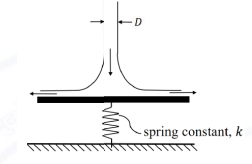
\includegraphics[width=0.5\columnwidth]{Figs/image (52).png}
\caption*{}
\label{fig:47}
\end{figure}

If the spring shows a steady deflection of $1~\text{cm}$ upon impingement of jet, then the velocity of the incoming jet is \underline{\hspace{2cm}}~m/s (\text{round off to one decimal place}).

\hfill{\brak{\text{GATE ME 2021}}}

\item A single jet Pelton wheel operates at $300$ rpm. The mean diameter of the wheel is $2$ m. Operating head and dimensions of jet are such that water comes out of the jet with a velocity of $40~\text{m/s}$ and flow rate of $5~\text{m}^3/\text{s}$. The jet is deflected by the bucket at an angle of $165^\degree$. Neglecting all losses, the power developed by the Pelton wheel is \underline{\hspace{2cm}}~MW (\text{round off to two decimal places}).

\hfill{\brak{\text{GATE ME 2021}}}

\item An air-conditioning system provides a continuous flow of air to a room using an intake duct and an exit duct, as shown in the figure. To maintain the quality of the indoor air, the intake duct supplies a mixture of fresh air with a cold air stream. The two streams are mixed in an insulated mixing chamber located upstream of the intake duct. Cold air enters the mixing chamber at $5^\degree$C, $105$ kPa with a volume flow rate of $1.25~\text{m}^3/\text{s}$ during steady state operation. Fresh air enters the mixing chamber at $34^\degree$C and $105$ kPa. The mass flow rate of the fresh air is $1.6$ times of the cold air stream. Air leaves the room through the exit duct at $24^\degree$C.
\begin{figure}[h]
\centering
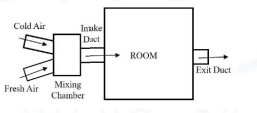
\includegraphics[width=0.5\columnwidth]{Figs/image (53).png}
\caption*{}
\label{fig:49}
\end{figure}
Assuming the air behaves as an ideal gas with $C_p = 1.005~\text{kJ/kg.K}$ and $R = 0.287~\text{kJ/kg.K}$, the rate of heat gain by the air from the room is \underline{\hspace{2cm}}~kW (\text{round off to two decimal places}).

\hfill{\brak{\text{GATE ME 2021}}}

\item Two smooth identical spheres each of radius $125~\text{mm}$ and weight $100~\text{N}$ rest in a horizontal channel having vertical walls. The distance between vertical walls of the channel is $400~\text{mm}$.
\begin{figure}[h]
\centering
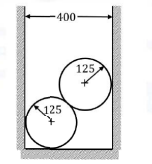
\includegraphics[width=0.5\columnwidth]{Figs/image (54).png}
\caption*{}
\label{fig:50}
\end{figure}
The reaction at the point of contact between two spheres is \underline{\hspace{2cm}}~N (\text{round off to one decimal place}).

\hfill{\brak{\text{GATE ME 2021}}}

\item An overhanging beam $PQR$ is subjected to uniformly distributed load $20~\text{kN/m}$ as shown in the figure.
\begin{figure}[h]
\centering
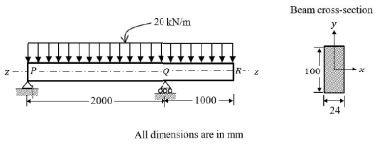
\includegraphics[width=0.5\columnwidth]{Figs/image (55).png}
\caption*{}
\label{fig:51}
\end{figure}

The maximum bending stress developed in the beam is \underline{\hspace{2cm}}~MPa (\text{round off to one decimal place}).

\hfill{\brak{\text{GATE ME 2021}}}

\item The Whitworth quick return mechanism is shown in the figure with link lengths as follows: $OP=300$ mm, $OA=150$ mm, $AR=160$ mm, $RS=450$ mm
\begin{figure}[h]
\centering
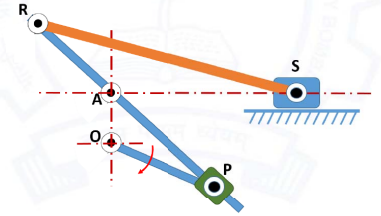
\includegraphics[width=0.5\columnwidth]{Figs/image (56).png}
\caption*{}
\label{fig:52}
\end{figure}

The quick return ratio for the mechanism is \underline{\hspace{2cm}} (\text{round off to one decimal place}).

\hfill{\brak{\text{GATE ME 2021}}}

\item A short shoe drum (radius $260$ mm) brake is shown in the figure. A force of $1~\text{kN}$ is applied to the lever. The coefficient of friction is $0.4$.
\begin{figure}[h]
\centering
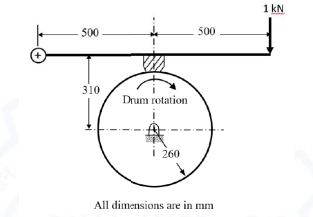
\includegraphics[width=0.5\columnwidth]{Figs/image (57).png}
\caption*{}
\label{fig:53}
\end{figure}

The magnitude of the torque applied by the brake is \underline{\hspace{2cm}}~N.m (\text{round off to one decimal place}).

\hfill{\brak{\text{GATE ME 2021}}}

\item A machine part in the form of cantilever beam is subjected to fluctuating load as shown in the figure. The load varies from $800~\text{N}$ to $1600~\text{N}$. The modified endurance, yield and ultimate strengths of the material are $200~\text{MPa}$, $500~\text{MPa}$ and $600~\text{MPa}$, respectively.
\begin{figure}[h]
\centering
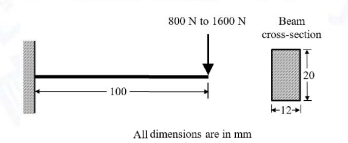
\includegraphics[width=0.5\columnwidth]{Figs/image (58).png}
\caption*{}
\label{fig:54}
\end{figure}
The factor of safety of the beam using modified Goodman criterion is \underline{\hspace{2cm}} (\text{round off to one decimal place}).

\hfill{\brak{\text{GATE ME 2021}}}


\item A cantilever beam of rectangular cross-section is welded to a support by means of two fillet welds as shown in figure. A vertical load of $2$~kN acts at free end of the beam.
\begin{figure}[h]
\centering
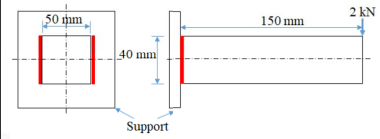
\includegraphics[width=0.5\columnwidth]{Figs/image (59).png}
\caption*{}
\label{fig:55}
\end{figure}
Considering that the allowable shear stress in weld is $60~\text{N/mm}^2$, the minimum size (leg) of the weld required is \underline{\hspace{2cm}}~mm (\text{round off to one decimal place}).

\hfill{\brak{\text{GATE ME 2021}}}

\end{enumerate}

\end{document}